\documentclass[11pt,letterpaper]{article}

% Load some basic packages that are useful to have
% and that should be part of any LaTeX installation.
%
% be able to include figures
\usepackage{graphicx}
% get nice colors
\usepackage{xcolor}

% change default font to Palatino (looks nicer!)
\usepackage[latin1]{inputenc}
\usepackage{mathpazo}
\usepackage[T1]{fontenc}
% load some useful math symbols/fonts
\usepackage{latexsym,amsfonts,amsmath,amssymb}

% comfort package to easily set margins
\usepackage[top=1in, bottom=1in, left=1in, right=1in]{geometry}

% control some spacings
%
% spacing after a paragraph
\setlength{\parskip}{.15cm}
% indentation at the top of a new paragraph
\setlength{\parindent}{0.0cm}


\begin{document}

\begin{center}
\Large
Ay190 -- Worksheet 2\\
Anthony Alvarez\\
Date: \today
\end{center}

\section{An Unstable Calculation}

Consider the following sequence and recurrence relation 

$$ x_0 = 1;\ x1=\frac{1}{3},\ x_{n+1} = \frac{13}{3} x_n - \frac{4}{3}x_{n-1},$$

which is equivalent to 

$$ x_n = \left( \frac{1}{3} \right)^n .$$

In the recurence relation at $n = 15$ we have quite a large error. With the
recursive realtion we get that $\frac{1}{3} ^ {15} =0.914373$ while the 
{\it true} value is $6.9692 10 ^{-8}$.  The absolute error is $-0.9008$ and 
the relative error is $-4308627.0610$.

\section{Finite Difference Approximation and Convergence}

\subsection{Forward Differencing}

\begin{figure}[bth]
\centering
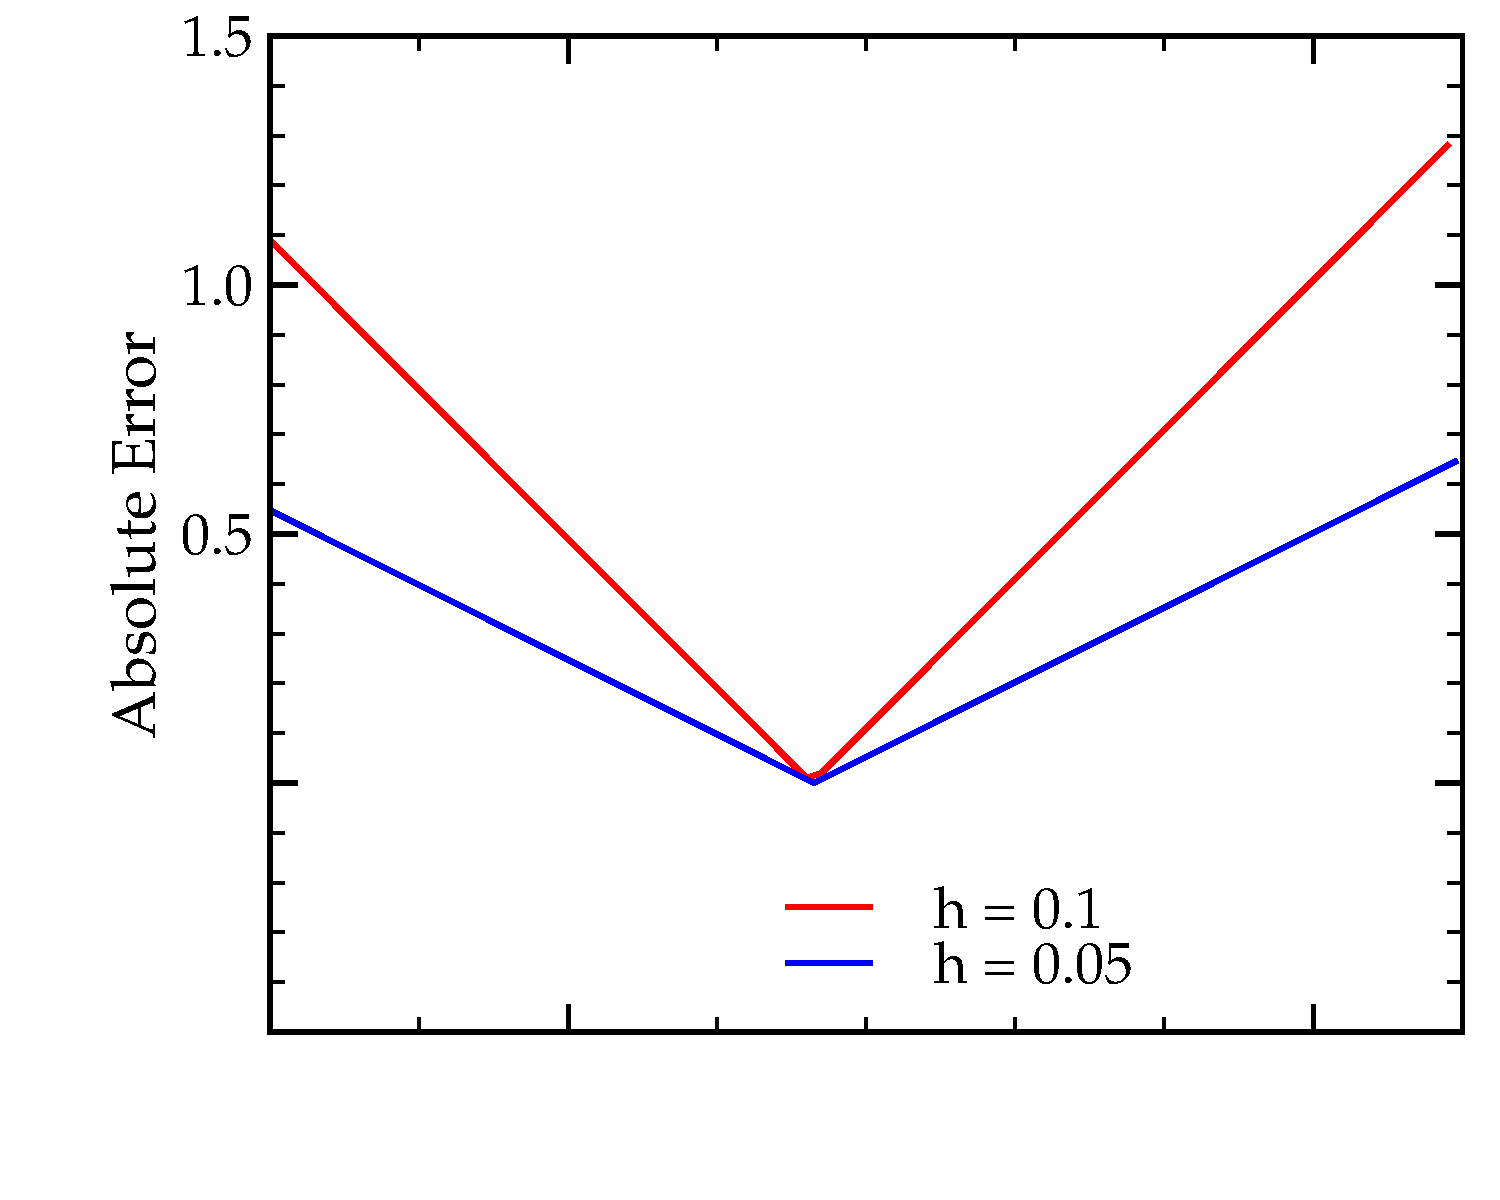
\includegraphics[width=0.5\textwidth]{forward_difference.pdf}
\caption{Absolute Error with Forward Differencing on the function $f(x) = 
x^3 -5x^2+x$.}
\label{fig:forward_difference}
\end{figure}

In figure~\ref{fig:forward_difference} we see that the forward differencing is
first order convergent since by halving h we half the absolute error.

\subsection{Central Differencing}


\begin{figure}[bth]
\centering
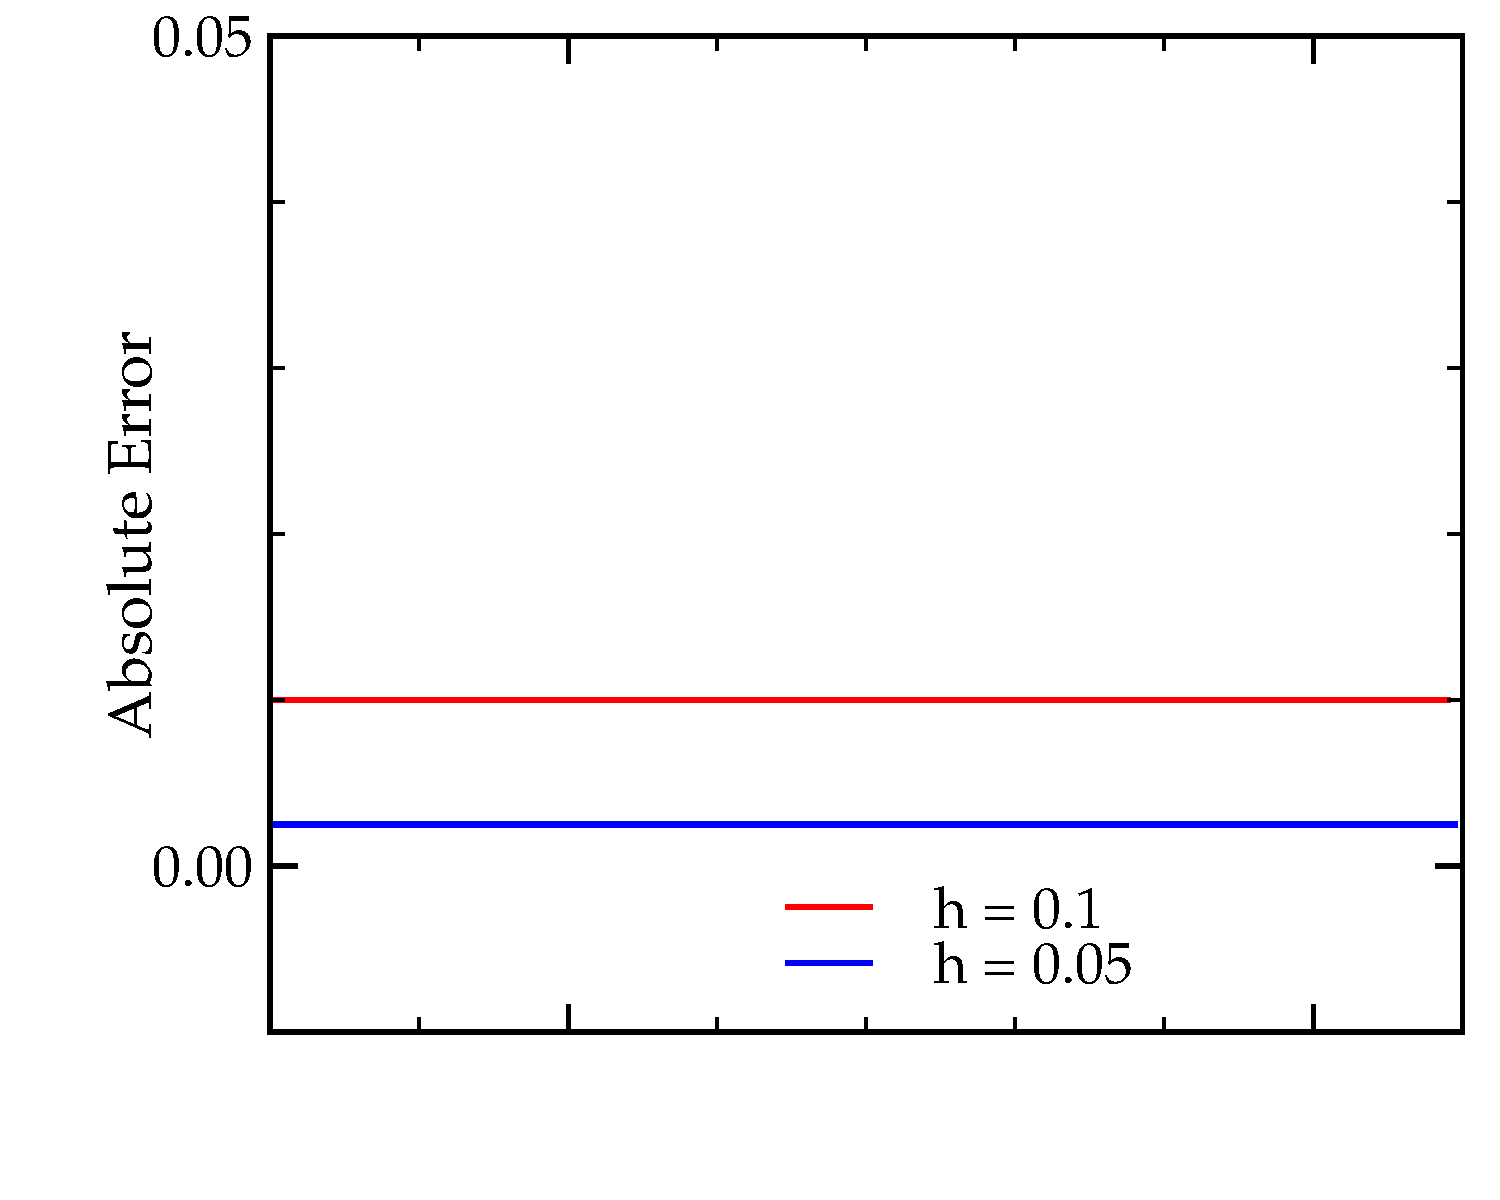
\includegraphics[width=0.5\textwidth]{central_difference.pdf}
\caption{Absolute Error with Central Differencing on the function $f(x) = 
x^3 -5x^2+x$.}
\label{fig:central_difference}
\end{figure}

In figure~\ref{fig:central_difference} we see that the central differencing is
second order convergent since by halving h we quarter the absolute error. It's 
also interesting to note that for this particular function the central
differencing scheme produces constant absolute error.

\section{Second Derivative}

$$f''(x) = \lim_{h \to 0}\frac{f'(x+h) - f'(x-h)}{2h}$$

We know that $f'(x)$ when calcualted using central diffferencing is second
order. So we plug in 
$$f'(x) \lim_{h \to 0} \frac{f(x+h) - f(x-h)}{2h}$$ 

giving

$$f''(x) = \lim_{h \to 0}
    \frac{\left(f(x+2h) - f(x)\right) - \left( f(x) + f(x-2h)\right)}{4h^2}$$

$$f''(x) = \lim_{h \to 0}\frac{f(x+2h) - 2f(x) + f(x-2h)}{4h^2}$$

This is a second-order central finite difference approximation for the second
derivative of the function $f(x)$ assuming a fixed step size h.

\section{Interpolation: Cepheid Lightcurve}

\subsection{Lagrange Interpolation}
\begin{figure}[bth]
\centering
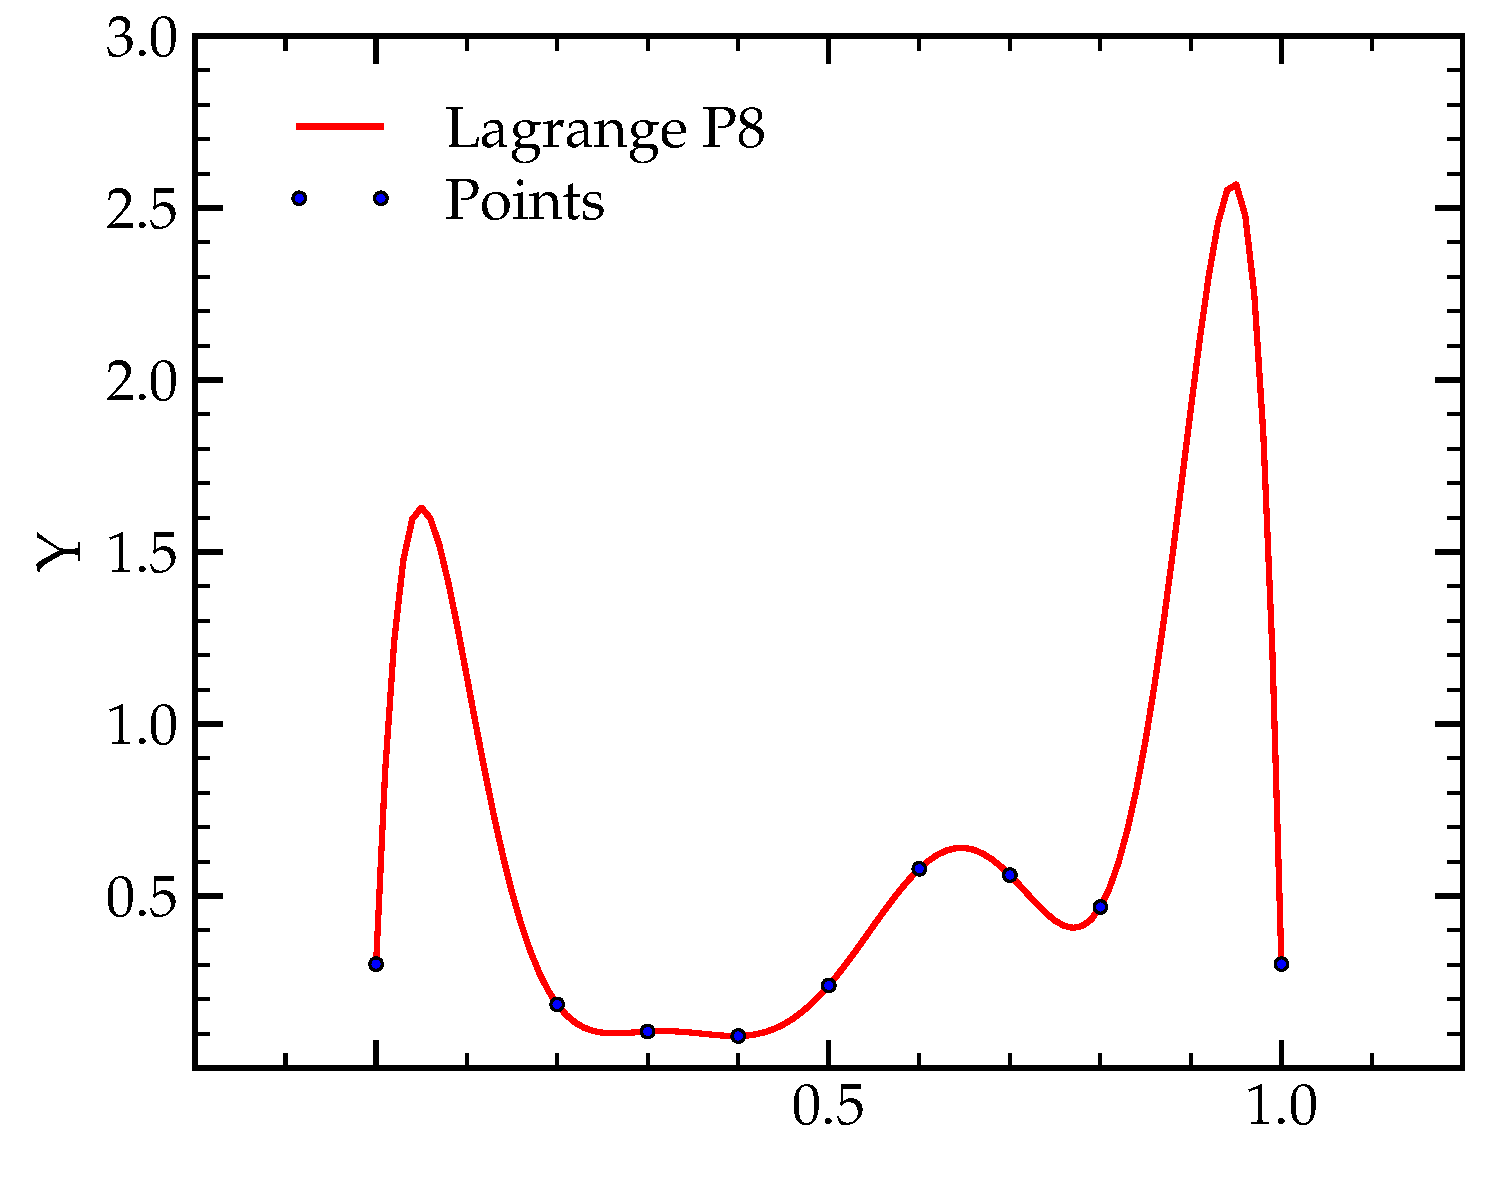
\includegraphics[width=0.5\textwidth]{lagrange.pdf}
\caption{Lagrange interpolation polynomial $p_8(x)$ and the data together.}
\label{fig:lagrange}
\end{figure}

In figure~\ref{fig:lagrange} we can see the Runge's phenomenon of 
non-convergence on the edges where the data gets a bit sparce. 

\subsection{Piecewise Linear \& Quadratic Interpolation}

\begin{figure}[bth]
\centering
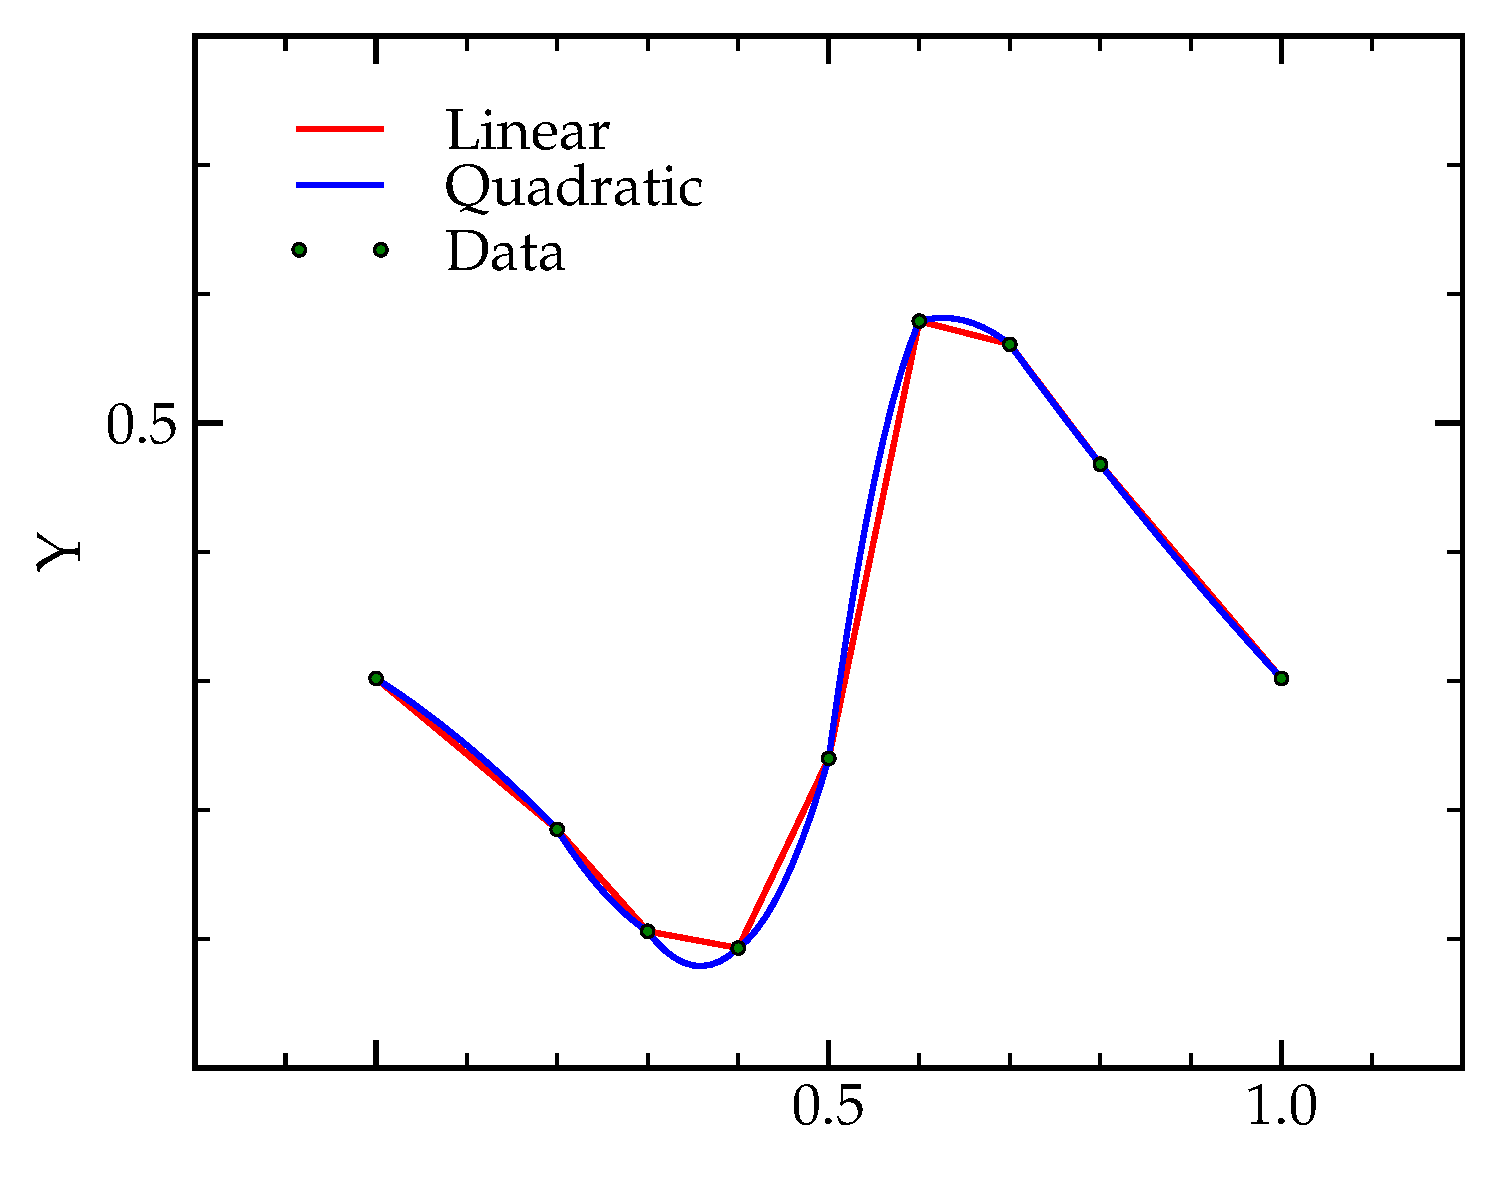
\includegraphics[width=0.5\textwidth]{lin_quad.pdf}
\caption{Piecewise linear and quadratic interpolation and the data together.}
\label{fig:lin_quad}
\end{figure}

In figure~\ref{fig:lin_quad} we can see the linear and quadratic model match the
data better than the Lagrange interpolation scheme. Also we note that the 
quadratic model is smoother, as one would expect.

\section{More Cepheid Lightcurve Interpolation}

\subsection{Piecewise Cubic Hermite \& Natural Cubic Spline Interpolation}

\begin{figure}[bth]
\centering
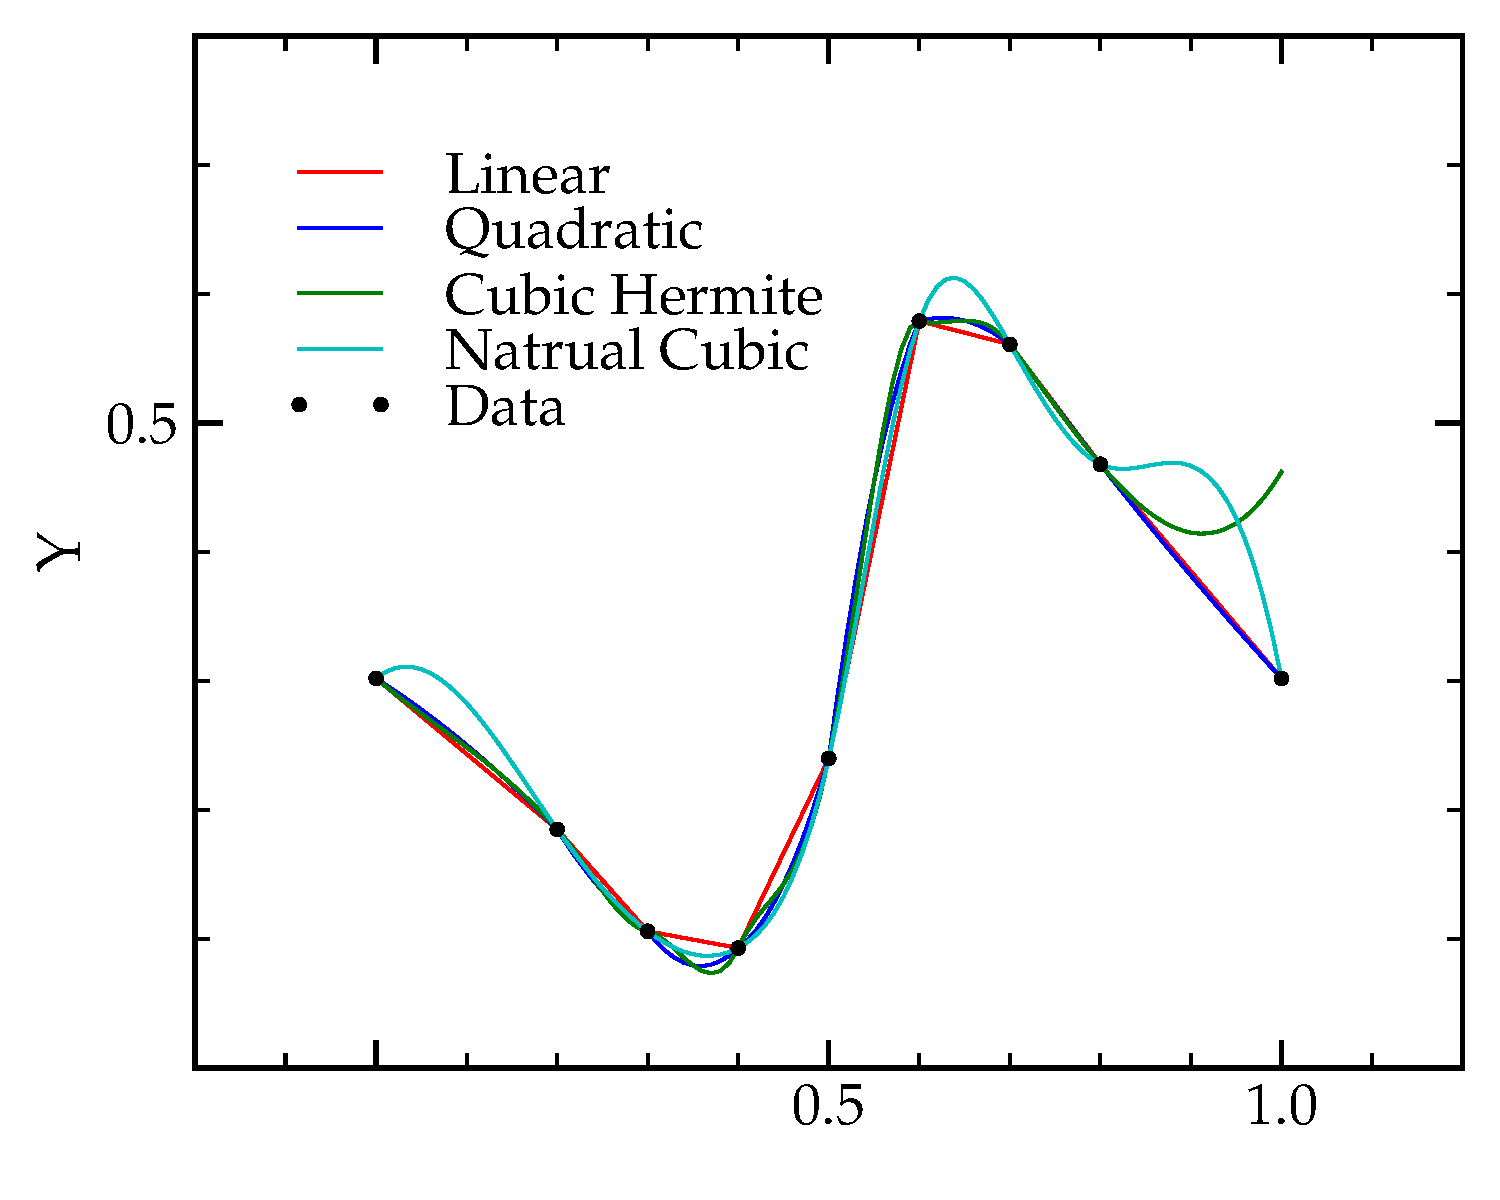
\includegraphics[width=0.5\textwidth]{herm_natural_cubic.pdf}
\caption{Piecewise Linear, Quadratic, Cubic Hermite, Natural Cubic Spline
Interpolation \& the data itself.}
\label{fig:herm_natural}
\end{figure}

In figure~\ref{fig:herm_natural} we can see that the Natural Cubic Spline
is the smoothest of the interpolations. We also note that the Cubic Hermite 
has strange behavior in the last bin. This is due to the fact that we cannot 
numerically calculate the derivative on the right edge so this is infact not
an interpolation but actually an extrapolation.


\end{document}
